\documentclass{article}
\usepackage[UKenglish]{babel}

\usepackage{graphicx}
\usepackage{booktabs}
\usepackage{multirow}
\usepackage{amsmath}
\usepackage{natbib}
\usepackage{color}

%\usepackage[paperwidth=15.75cm, paperheight=5cm, margin=0cm]{geometry}
\usepackage[paperwidth=174mm, paperheight=80mm, margin=0cm]{geometry}
\renewcommand{\familydefault}{\sfdefault}
\setlength\parindent{0pt}

\begin{document}
\hspace{-1em}
\begin{tabular}{l@{\hspace{5mm}}r}
  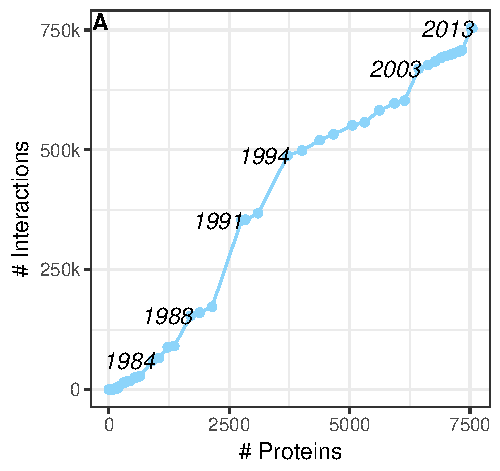
\includegraphics{Figure2a.pdf}&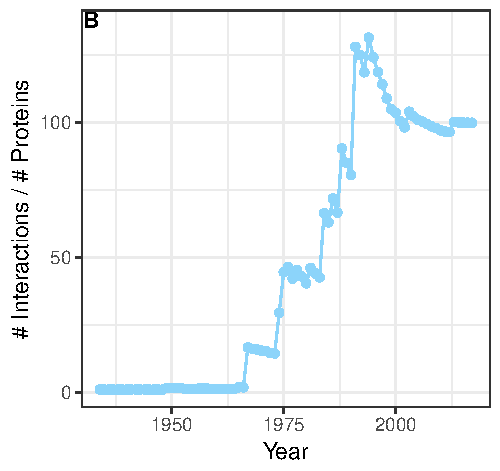
\includegraphics{Figure2b.pdf}
\end{tabular}
\end{document}
